\documentclass[12pt,letterpaper]{article}

\usepackage[portrait]{geometry}
\geometry{tmargin=1in,bmargin=1in,lmargin=1in,rmargin=1in}
\usepackage{graphicx}
\usepackage{amsmath}
%\usepackage{../latex/lplfitch}
\usepackage{enumitem}
\usepackage{color}

\usepackage{fancyvrb}
\usepackage{listings}
\usepackage{lstautogobble}

\lstset{basicstyle=\ttfamily,
  mathescape=true,
  escapeinside=||,
  autogobble}

\usepackage{fancyhdr}
\pagestyle{fancy}

\lhead{\Large{\bf Assignment 9}}
\chead{}
\rhead{}
\lfoot{CS 375 - Analysis of Algorithms}
\cfoot{}
\rfoot{Page \thepage}
\renewcommand{\headrulewidth}{3pt}
\renewcommand{\footrulewidth}{3pt}
\usepackage{hyperref}
\usepackage{tikz}
\usetikzlibrary{automata,positioning}

\begin{document}
Recall the statement of the Ford-Fulkerson algorithm as follows: 
\begin{lstlisting}
    def residualGraph(graph $G$, flow $f$):
        Initialize a new graph $G_f$ with the same vertices as $G$
        for each edge $e$ in $G$:
            Let $e^{G_f}$ denote the corresponding edge in $G_f$
            Set $c_{e^{G_f}} = c_e - f(e)$
            If $f(e) > 0$:
                Let $e^R$ denote the reverse edge of $e^{G_f}$.
                Set $c_{e^R} = f(e)$.
        return $G_f$
    
    def FordFulkerson($G$, $s$, $t$):
        Initialize $f$ as zero flow. 
        while there is an $s\rightarrow t$ path $P$ in $G_f$ where the minimum 
                capacity $c$ over all the edges in $P$ is bigger 
                than 0:
            Set $f(e)$ += $c$ for all edges $e$ in $P$.
    
\end{lstlisting}
Trace through the \texttt{FordFulkerson} algorithm on the following input:
\begin{center}
    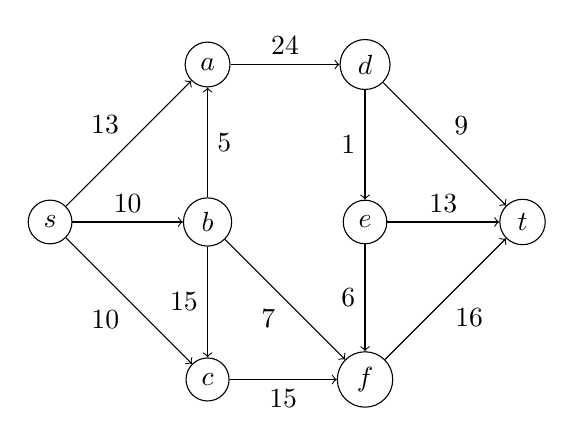
\begin{tikzpicture}
        \node[draw, circle] (s) at (0, 0) {$s$};
        \node[draw, circle] (a) at (2, 2) {$a$};
        \node[draw, circle] (b) at (2, 0) {$b$};
        \node[draw, circle] (c) at (2, -2) {$c$};
        \node[draw, circle] (d) at (4, 2) {$d$};
        \node[draw, circle] (e) at (4, 0) {$e$};
        \node[draw, circle] (f) at (4, -2) {$f$};
        \node[draw, circle] (t) at (6, 0) {$t$};
        
        \draw[->] (s) -- (a) node[midway, above left] {13};
        \draw[->] (s) -- (b) node[midway, above] {10};
        \draw[->] (s) -- (c) node[midway, below left] {10};
        \draw[->] (b) -- (a) node[midway, right] {5};
        \draw[->] (b) -- (c) node[midway, left] {15};
        \draw[->] (a) -- (d) node[midway, above] {24};
        \draw[->] (b) -- (f) node[midway, below left] {7};
        \draw[->] (c) -- (f) node[midway, below] {15};
        \draw[->] (d) -- (e) node[midway, left] {1};
        \draw[->] (e) -- (f) node[midway, left] {6};
        \draw[->] (d) -- (t) node[midway, above right] {9};
        \draw[->] (e) -- (t) node[midway, above] {13};
        \draw[->] (f) -- (t) node[midway, below right] {16};
    \end{tikzpicture}
\end{center}
After determining the maximum flow, find am $s$-$t$ cut with equal cut value. 
\end{document}